% THIS IS SIGPROC-SP.TEX - VERSION 3.1
% WORKS WITH V3.2SP OF ACM_PROC_ARTICLE-SP.CLS
% APRIL 2009
%
% It is an example file showing how to use the 'acm_proc_article-sp.cls' V3.2SP
% LaTeX2e document class file for Conference Proceedings submissions.
% ----------------------------------------------------------------------------------------------------------------
% This .tex file (and associated .cls V3.2SP) *DOES NOT* produce:
%       1) The Permission Statement
%       2) The Conference (location) Info information
%       3) The Copyright Line with ACM data
%       4) Page numbering
% ---------------------------------------------------------------------------------------------------------------
% It is an example which *does* use the .bib file (from which the .bbl file
% is produced).
% REMEMBER HOWEVER: After having produced the .bbl file,
% and prior to final submission,
% you need to 'insert'  your .bbl file into your source .tex file so as to provide
% ONE 'self-contained' source file.
%
% Questions regarding SIGS should be sent to
% Adrienne Griscti ---> griscti@acm.org
%
% Questions/suggestions regarding the guidelines, .tex and .cls files, etc. to
% Gerald Murray ---> murray@hq.acm.org
%
% For tracking purposes - this is V3.1SP - APRIL 2009

\documentclass{acm_proc_article-sp}

\begin{document}

\title{Data Prognostics Using Symbolic Regression}
\subtitle{An Effort to Characterize Turbofan Engine Degradation}
%\titlenote{A full version of this paper is available as
%\textit{Author's Guide to Preparing ACM SIG Proceedings Using
%\LaTeX$2_\epsilon$\ and BibTeX} at
%\texttt{www.acm.org/eaddress.htm}}}
%
% You need the command \numberofauthors to handle the 'placement
% and alignment' of the authors beneath the title.
%
% For aesthetic reasons, we recommend 'three authors at a time'
% i.e. three 'name/affiliation blocks' be placed beneath the title.
%
% NOTE: You are NOT restricted in how many 'rows' of
% "name/affiliations" may appear. We just ask that you restrict
% the number of 'columns' to three.
%
% Because of the available 'opening page real-estate'
% we ask you to refrain from putting more than six authors
% (two rows with three columns) beneath the article title.
% More than six makes the first-page appear very cluttered indeed.
%
% Use the \alignauthor commands to handle the names
% and affiliations for an 'aesthetic maximum' of six authors.
% Add names, affiliations, addresses for
% the seventh etc. author(s) as the argument for the
% \additionalauthors command.
% These 'additional authors' will be output/set for you
% without further effort on your part as the last section in
% the body of your article BEFORE References or any Appendices.

\numberofauthors{1} %  in this sample file, there are a *total*
% of EIGHT authors. SIX appear on the 'first-page' (for formatting
% reasons) and the remaining two appear in the \additionalauthors section.
%
\author{
% You can go ahead and credit any number of authors here,
% e.g. one 'row of three' or two rows (consisting of one row of three
% and a second row of one, two or three).
%
% The command \alignauthor (no curly braces needed) should
% precede each author name, affiliation/snail-mail address and
% e-mail address. Additionally, tag each line of
% affiliation/address with \affaddr, and tag the
% e-mail address with \email.
%
% 1st. author
\alignauthor
V. Hunter Adams\\
       \affaddr{Cornell University}\\
       \email{vha3@cornell.edu}
}
% There's nothing stopping you putting the seventh, eighth, etc.
% author on the opening page (as the 'third row') but we ask,
% for aesthetic reasons that you place these 'additional authors'
% in the \additional authors block, viz.

% Just remember to make sure that the TOTAL number of authors
% is the number that will appear on the first page PLUS the
% number that will appear in the \additionalauthors section.

\maketitle
\begin{abstract}

What follows is an application of symbolic regression to sensor output from a fleet of failing turbofan engines. The goal is to characterize engine failure, and then to use that characterization for predicting the remaining lifetimes and the moments of failure for engines in a separate fleet.

The genetic program makes the assumption that engine degradation manifests itself as changing correlations between sensor outputs, and searches for those correlations by evolving functions for remaining lifetime in terms of sensor outputs. NASA provides a training set in which 100 simulated engines are run to failure, and a test set in which a separate set of 100 simulated engines are shut off before they fail \cite{nasa}. The goal is to use information learned in the training set to predict the remaining lifetime of each engine in the test set.

Moghaddass and Zuo of the University of Alberta performed a similar analysis using a different technique that provides a baseline \cite{Mog}. The genetic program matched their technique and was able to characterize the moment of failure for every engine in the fleet. Moghaddass and Zuo's plots are included below for empirical comparison.


\end{abstract}



\section{Introduction}
In complex engineering projects such as turbine development, there is a huge demand for low-cost health monitoring systems. Failure of machines like these leads to extremely expensive (or dangerous) downtime, and data prognostics methods like the one presented here offer a means for mitigating risk by detecting degradation before failure occurs.\cite{Mog}

Prognostic health monitoring is an area of very active research and has been approached from a number of different perspectives. Moghaddass and Zuo used a machine learning approach. They characterized engine degradation as a multistage process and treated the prognostics process as a classification problem that places each engine in a particular phase of degradation \cite{Mog}. Others have approached the problem using belief functions, neural network based particle filtering, and hidden Markov models. \cite{nasa} \cite{oil}.

There is a lot of precedence for using symbolic regression to characterize physical systems. Dr. Hod Lipson has used this technique for determining system equations of motion \cite{symbolic}, and Byington et. al. of Impact Technologies used symbolic regression on spectroscopy data to evaluate the health of diesel engine lubricating oil \cite{oil}. Eureqa by Nutonian, software developed under the advisory of Dr. Hod Lipson, uses symbolic regression to find relationships in complex data sets \cite{nutonian}. Symbolic regression has not been applied to this problem specifically, but its similarity to those mentioned above suggest that it would be a promising technique. 

Symbolic regression was also well suited for the particular question that I intended to answer.  I searched for an integer corresponding to the number of cycles remaining in the engine. The answer to this question would take the form of a function of sensor output, which is a structure that symbolic regression accommodates very well.


I baselined performance of my own algorithm against that of Maghoaddas and Zuo, whose plots are included below for comparison with my own \cite{Mog}. The genetic program matched Maghoaddas and Zuo in predictive capability, and it was able to identify the moments of failure for each engine in the test dataset.


\section{Problem Definition}
The input to the system is sensor data from 100 engines. Each engine has 26 sensors that, for the training data set, record information until the engine fails. The output of the system is a single number for each engine, which corresponds to that engine's remaining lifetime.


To be clear, the program evolves function of the form:

\begin{equation}
L_{remaining} = f (sensor_{i}, sensor_{j}, sensor_{k}, \dots )
\end{equation}

Where $L_{remaining}$ is remaining engine lifetime, which may be a function of any combination of some or all of the sensors.

It is worth noting that the program is entirely system agnostic. It treats all sensors purely as sources of data and has no information about what the data means physically.

\section{Method}
Because this is a genetic algorithm, it deals with a population of solutions. For each generation, the population goes through five distinct steps, each of which will be elaborated upon in the subsections \cite{class}. These steps include:

\begin{enumerate}
\item Rank the population according to fitness criteria
\item Select subset of the population that will survive/breed in the next generation
\item Perform crossover among the surviving parent population to create a population of children
\item Perform mutation on the child population
\item Add the child population to the parent population to replenish the original population size
\item Return to step 1
\end{enumerate}

The subtleties of each step are discussed below.

\subsection{Rank the Population}
In order to maintain genetic diversity in the population, I used elitist multi objective optimization on a Pareto front \cite{class}. The solutions in the population were optimized along four dimensions:

\begin{itemize}
\item {\underline{Age}}: Solutions that have been in the population for a shorter amount of time are more fit (in the age dimension) than solutions that have been evolving for a long time. This helps maintain diversity in the population by giving solutions with more potential to evolve an advantage over those that have become stagnant. During crossover, the child adopts the age of its oldest parent. \cite{class}
\item {\underline{Mean Prediction Error}}: Solutions that have a lower average prediction error (measured across all engines in the fleet) are more fit than solutions that have higher average error.
\item {\underline{Uniqueness}}: Solutions that have good predictability on particular engines that other members of the population are unable to predict are more fit in the uniqueness dimension. This helps maintain diversity.
\item {\underline{Worst Prediction}}: Solutions with lower error on their worst prediction are more fit than solutions with higher error on their worst prediction (even if they have a lower mean error over all engines). This prevents the algorithm from getting stuck at the mean remaining lifetime of all engines in the fleet.
\end{itemize}

The solutions that compose the population are placed on a series of Pareto fronts according to the NSGA non-dominated sort laid out by Seshadri in \cite{pareto}. In brief, the population is sorted in the following way:

\begin{enumerate}
\item Initialize the {\it{number}} of individuals that dominate each member of the population to 0 and the {\it{members of the population}} that each member of the population dominates to an empty list.
\item For each member of the population $p$, loop through every other member of the population $q$. If $p$ dominates $q$, then add $q$ to the list of solutions that $p$ dominates. If $q$ dominates $p$, then increment the domination counter by 1.
\item If the domination counter equals 0 for a particular solution, then add that solution to the leading Pareto front.
\item Initialize a second Pareto front as an empty list.
\item Decrement the domination counter for every solution by 1. If the domination counter for any of the solutions becomes 0, add it to the second Pareto front (because this means it was only dominated by one of the individuals in the first Pareto front).
\item Return to step 3 and continue until all solutions have been placed in a Pareto front
\end{enumerate}

Domination is defined as being the equally or more fit along each of the four dimensions of fitness (age, mean prediction error, uniqueness, and worst prediction), and more fit along any one of the dimensions. Once each solution is in a front, the algorithm moves on to the selection process \cite{horn}.

\begin{figure}[!h]
\center
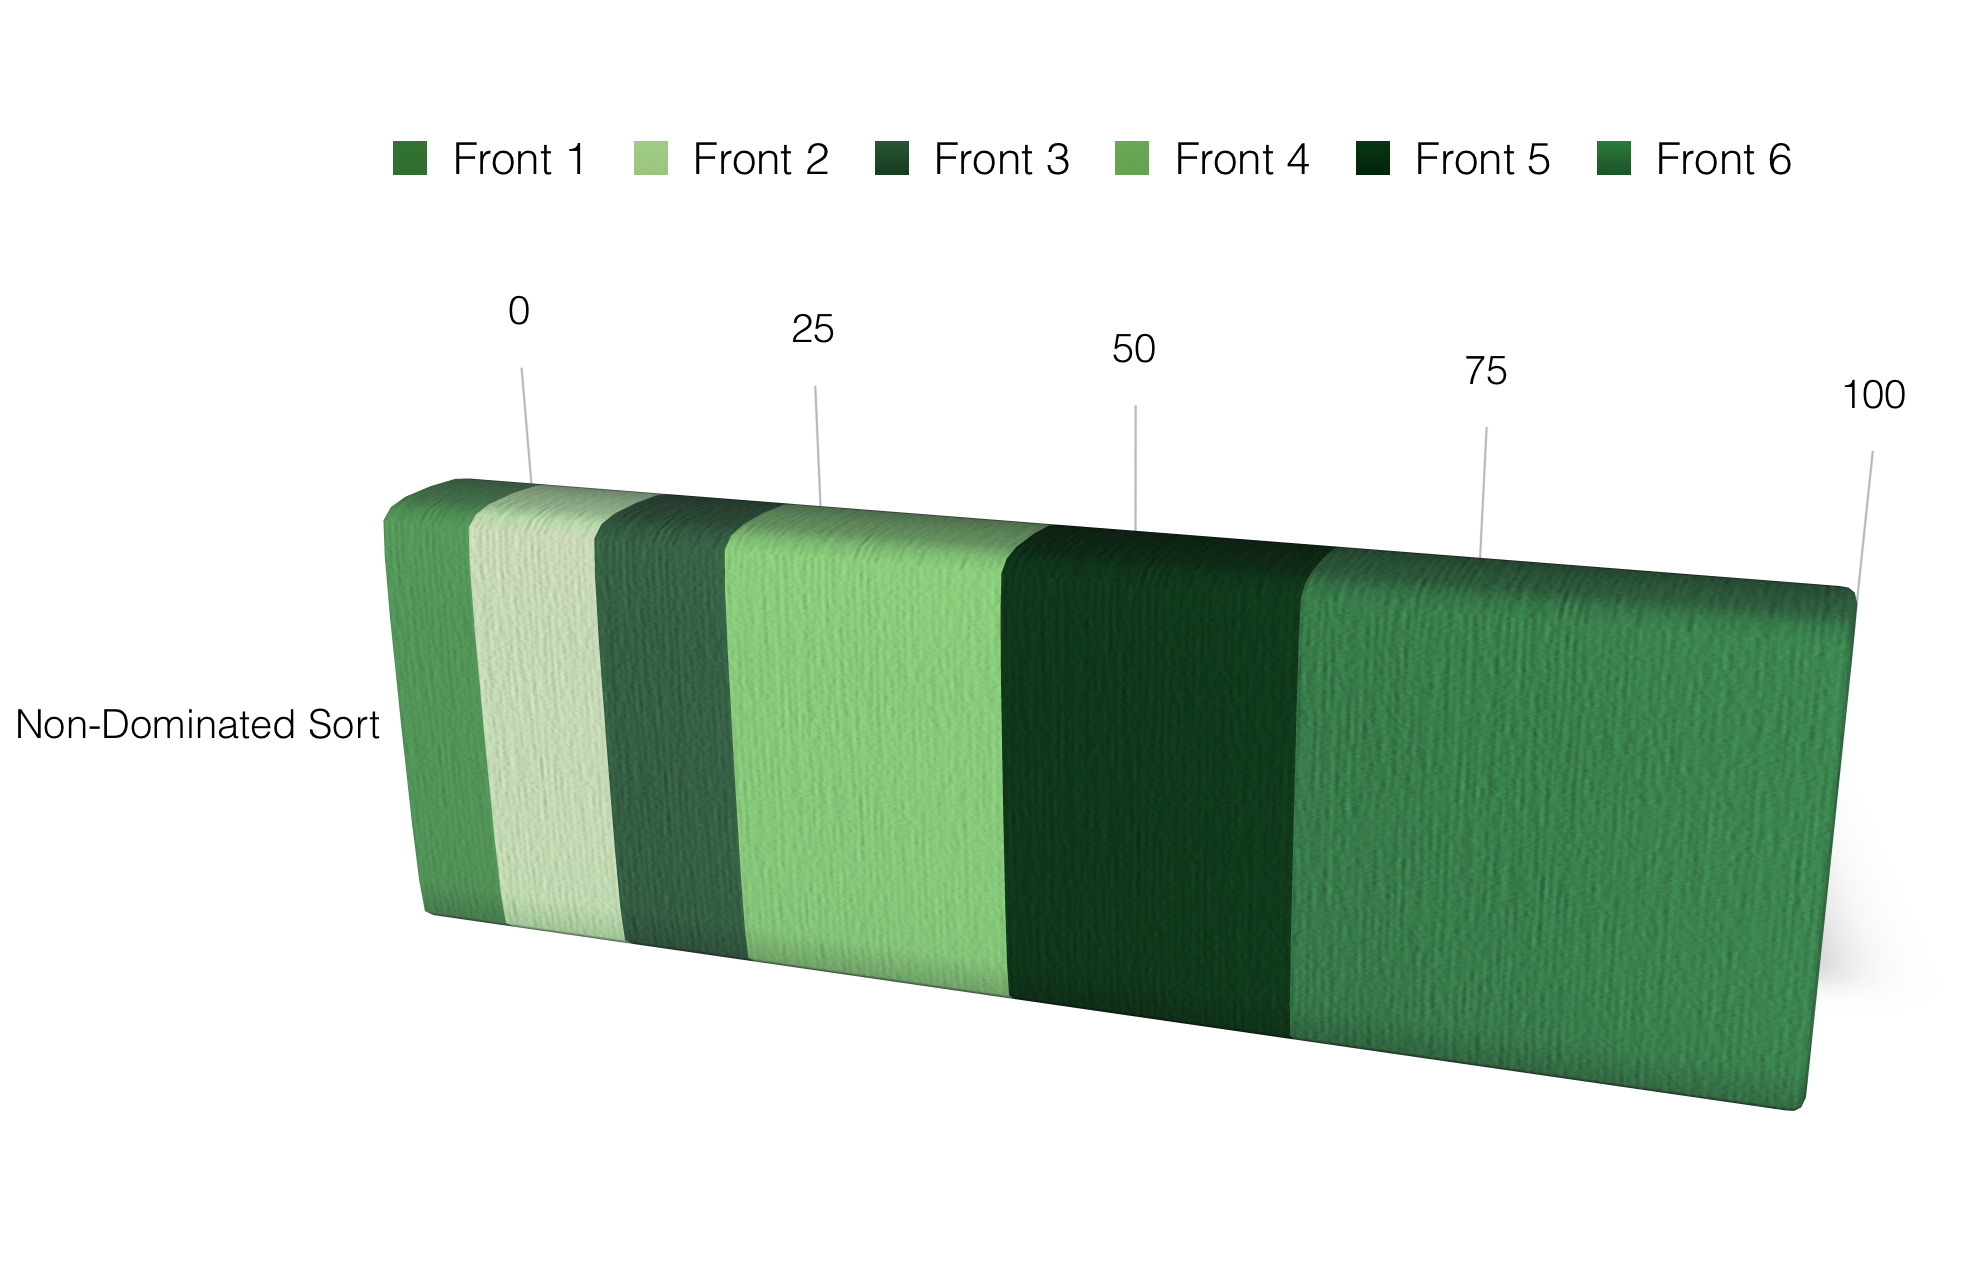
\includegraphics[scale=0.25]{Fronts.png}
\caption {A visualization of how the population is divided into fronts. The relative sizes of the fronts change from generation to generation.}
\label{fig:bullet}
\end{figure}


\subsection{Selection}
The algorithm uses elitism in that any solution that lives in the first Pareto front is guaranteed to survive into the next generation. All members of the population have some probability of surviving, but the solutions that occupy the more fit Pareto fronts have a higher probability of making it to the next generation.

The algorithm works with a selection pressure of 0.4 (empirically determined). I found that tighter selection pressures led to homogeneity in the population. After the members of the leading Pareto front were added to the surviving population, 80 percent of the remaining survivors were picked from the top 60 percent of the old population, and 20 percent of the remaining population were randomly generated {\it{new}} solutions that were added to the population. It was rare that any of these solutions had better predictive abilities than the older solutions that had been evolving, but because they were younger than the rest of the solutions a few were able to survive \cite{class}. This helped maintain diversity in the population.

\begin{figure}[!h]
\center
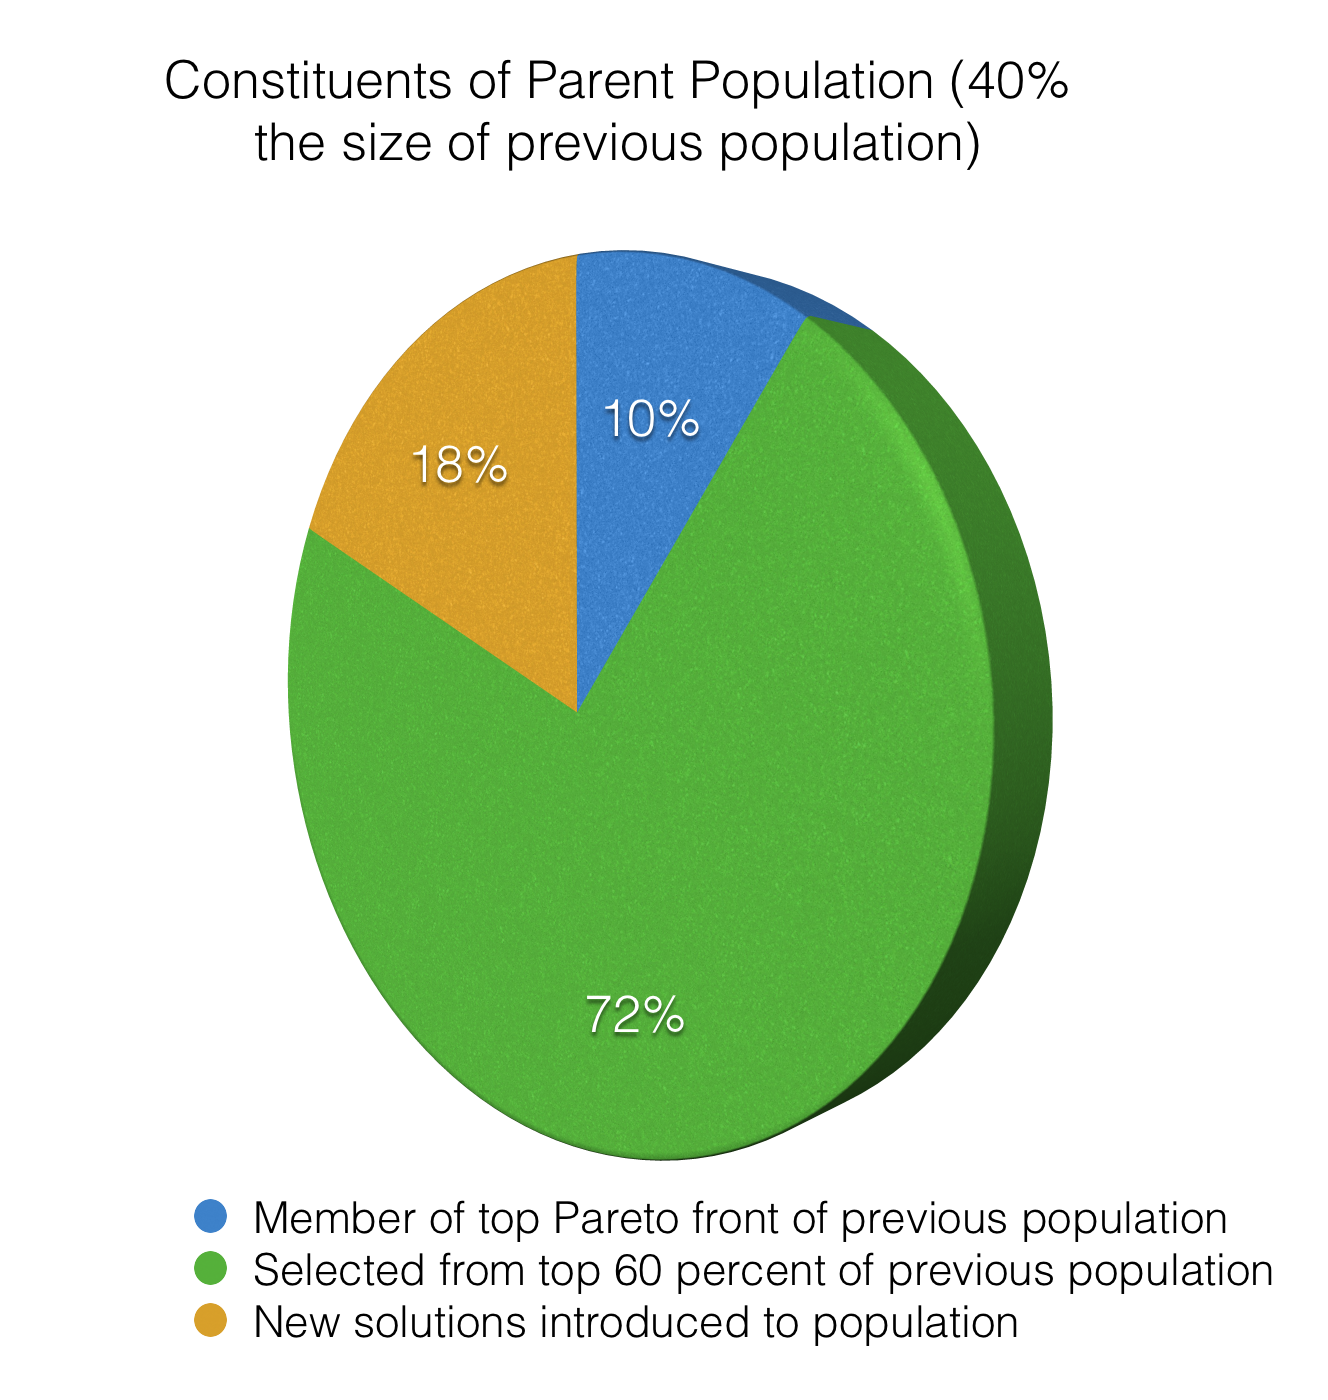
\includegraphics[scale=0.3]{Parent_Plot.png}
\caption {Constituent members of parent population after selection. The relative sizes change somewhat for each generation, depending on the size of the leading Pareto front.}
\label{fig:bullet}
\end{figure}



\subsection{Crossover}
In order to replenish the population to its original size, crossover was performed to produce child solutions from the surviving parent solutions. The mother preferred to be among the elite members of the population (ranked somewhere in the top 20), but the father was randomly selected from the parent population. I found that this practice led to useful diversity in the children. When both parents were randomly selected from the surviving population, I found that they produced very diverse children, none of whom were particularly fit.

Because the members of the population are functions that are represented as a tree structure, crossover amounts to swapping branches between parents to produce a new child that has traits of both mother and father \cite{symbolic}. The depth of crossover is randomly determined for each parent every time crossover occurs.

\begin{figure}[!h]
\center
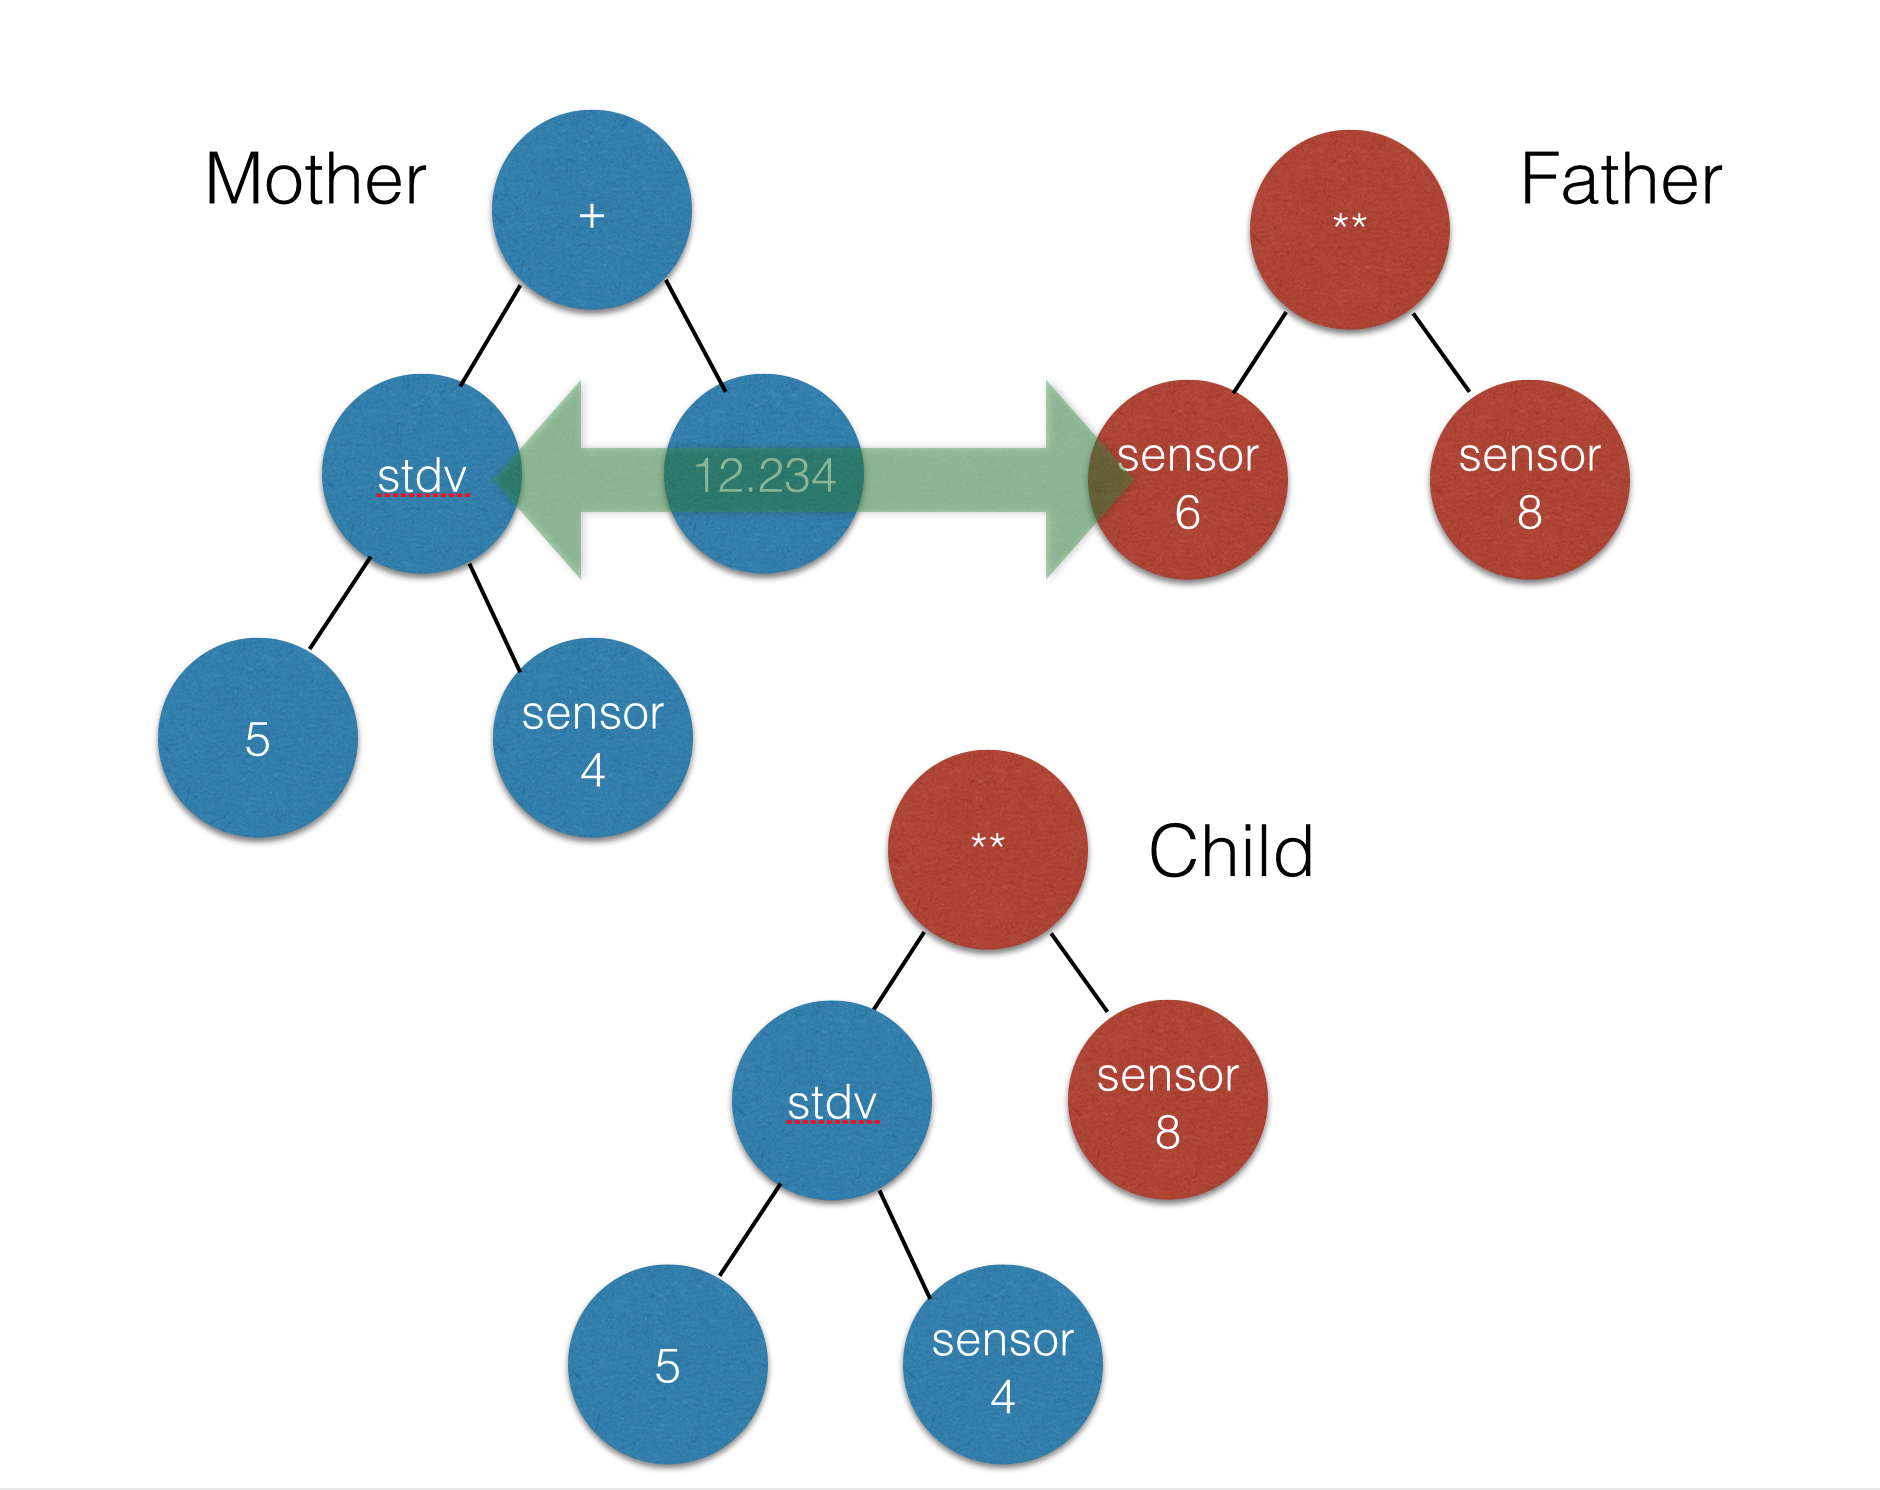
\includegraphics[scale=0.25]{crossover.png}
\caption {Two parent solutions producing a child solution by swapping branches.}
\label{fig:bullet}
\end{figure}

\subsection{Mutation}
After crossover creates a new child, it is mutated before being placed into the population. While crossover allows the population to strategically explore new parts of the optimization landscape, mutations are small variations that allow solutions to climb whichever peak they find themselves on. The mutations should not be disruptive to the good genes in the genome.

The mutation rate cools as the algorithm runs, until it reaches a particular number of generations (I found 100 worked well). At this point the mutation rate heats back up before cooling off again over the course of the next 100 generations. The algorithm had the ability to make the following mutations:

\begin{itemize}
\item Mutate the value of a constant
\item Change a constant to the output of a sensor
\item Change a sensor variable to a constant
\end{itemize}

The algorithm may not mutate operators, because this sort of mutation is often extremely disruptive to the existing genes.

\subsection{Replacement into Population}
In order to maintain diversity, I replace the children into the population using a form of deterministic crowding. After a child is created, the program checks whether it dominates either of its parents. If the child dominates a parent, then it replaces the parent.

Because the algorithm uses a cooling (and periodically heated up) mutation rate, there are a few generations for every 100 for which mutations are extremely rare. If crossover occurs between two solutions that are not very deep (contain very few branches), it is possible for the child to be identical to one of its parents. In order to prevent duplicate solutions in the population, every child is compared with every member of the population before being put into it. If a child does not replace a parent, and it is not identical to a solution that already lives in the population, then it enters the population.

\section{Related Work}
As mentioned in the introduction, data prognostics is an area of very active research that has been approached from a number of different directions. Moghaddass and Zuo applied a different sort of algorithm to this particular data set, while Dr. Lipson and the team at Nutonian tackled the general problem of data prognostics using a technique similar to that which I have implemented. \cite{Mog} \cite{nutonian}

Moghaddass and Zuo make the point that a multistage degradation can either be considered a continuous or a discrete process. By modeling degradation as a continuous process, one defines a threshold beyond which the machine is considered failed. In a discrete consideration of the same problem, the degradation process is quantized into discrete levels ranging from perfect operation to total failure. Traditionally, a discrete representation has been applied more to data diagnostics than data prognostics (that is, it answers the question "what is the current state of the machine?" rather than answering the question "how much longer until this machine fails?").  Moghaddass and Zuo are unique in that they did not assume a constant transition rate between states in order to estimate remaining engine lifetime, but they instead used non homogenous continuous-time semi-Markov processing for estimating the rate of transition between states. This allowed them to use traditional classification methods to place the engine in a particular state of degradation, and then estimate remaining lifetime based purely on its current state by estimating transition rates. Each state had an estimated probability of transitioning to another state in a given amount of time. \cite{Mog}

They are unfortunately a bit vague about the performance of their technique on the entire fleet of engines, instead providing plots of estimated remaining lifetime of 20 engines as evidence that the multistage structure is a reasonable structure of the degradation process. The plots do tell a compelling story, however, showing convergence on true remaining life for nearly all engines. \cite{Mog}

I elected to approach this problem using symbolic regression rather than the method explained above because I hoped to estimate a continuous variable (remaining engine lifetime) using continuous functions. While degradation may be a multi-stage process that is appropriately modeled discretely, remaining engine lifetime is fundamentally continuous. For this reason, I thought it would be interesting to attempt to answer this question using continuous representations. Additionally, Dr. Lipson and those at Nutonian have had a great deal of success approaching similar problems using a similar method. \cite{nutonian}

Eureka by Nutonian does almost precisely what I have attempted to do. It is a product that takes complex data sets as input, and uses symbolic regression to find relationships between particular data sources within the data set. Eureqa even offers the user the ability to "set a target," where he/she specifies the particular variable that should be modeled by the other variables in the data set. This is {\it{exactly}} the problem which I have attempted to solve myself. I ask for my genetic program to give me remaining engine lifetime as a function of the sensor outputs. \cite{nutonian}

Because Eureqa has been successful in solving similar types of problems, and because remaining engine lifetime is, by nature, a continuous variable; I have elected to apply the same techniques used by Nutonian to the particular problem of engine prognostics.

\section{System Architecture}
\subsection{Structure}
I have framed the problem in a machine learning context. The genetic program evolves tree data structures, where each node is an operator and each leaf is either a constant or an array of sensor output. The operators are arranged in a dictionary, and they include:

\begin{itemize}
\item {\underline{Arithmetic}}: Left leaf and right leaves are combined according to the arithmetic operator (+, -, *, /). These are four separate operators.
\item {\underline{Trigonometry}}: Left leaf is multiplied by the result of acting one of the three main trigonometric functions on the right leaf. These are three separate operators.
\item {\underline{Exponentiation}}: Left leaf is multiplied by the exponential of the right leaf.
\item {\underline{Logarithm}}: Left leaf is multiplied by the natural logarithm of the right leaf.
\item {\underline{Noise}}: Left leaf is multiplied by a Gaussian smear of the right leaf.
\item {\underline{Standard Deviation}}: Left leaf is multiplied by standard deviation of right leaf.
\item {\underline{Gradient}}: Left leaf is multiplied by gradient of right leaf.
\item {\underline{Second Gradient}}: Left leaf is multiplied by second gradient of right leaf.
\item {\underline{Window Operators}}: Left leaf is multiplied by one of the above 3 operators (standard deviation, gradient, or second gradient) acting only on the most recent 10 data points from the right leaf. These are three separate operators.
\end{itemize}

Sensor output is arranged in a separate dictionary, with each key corresponding to a separate engine and the value of each key being a list of 26 lists, each list corresponding to a different sensor. The GP evolves functions with the variables represented as keys of these dictionaries. When a function is evaluated for fitness (according to the criteria explained earlier), it is evaluated on every engine in the training fleet.

At a high level, the program works with objects of two classes. The "person" class is a tree structure like that I've just explained. An object of the person class has the ability to generate predictions for a particular engine, to evaluate its own depth, to perform crossover with another object of the person class, to mutate itself, to determine if it is dominant to another object of the person class, and to evaluate how good its predictions are on a particular engine. There are other methods associated with this class, but they are all helpers to these main methods.

The "population" class is, fundamentally, a list of objects of the person class. The population has the ability to perform operations on the population as a whole. It may add a person to the population, gather the traits of each member of the population (uniqueness, age, predictability, etc.), rank the population according to their traits, select a parent population from the entire population, and breed the members of the parent population to replenish its original size with children. These functions are combined to the broad "evolve()," "hillclimber()," and "randomSearch()" methods that attempt to maximize the fitness of the entire population.

As input, these broad optimization methods take mutation rate, population size, selection pressure, elitism pressure, and maximum allowable depth for the tree structures that compose the population.

\subsection{Data}
The data used for both training and testing comes from NASA's Prognostic Data Repository. Each dataset consists of 	multivariate time series, each variable corresponding to a different sensor or operational setting. The data was produced by C-MAPSS simulation software, which is the industry standard for simulating transient effects in turbofan engine degradation. For each engine in the training dataset, the engine starts under normal operation, develops a fault, and runs to failure \cite{nasa} \cite{Mog}. In the test dataset, the engines all start under normal operation, develop a fault, but are {\it{not}} run to failure. In particular, I have used dataset FD001, which is composed of engines of all the same type.

Minimal preprocessing was required for the genetic program to begin exploring the data. Each dataset was loaded into the python module and parsed into a dictionary. As explained previously, the key for each dictionary corresponds to a different engine, and the value of each key is a list of 26 lists corresponding to each sensor on the engine.

\section{Experimental Evaluation}
\subsection{Methodology}
The merit of each potential solution is judged in the training dataset alone. As previously discussed, the fitness of each member of the population is judged on a Pareto front that includes age, mean prediction error, uniqueness, and worst prediction. For sake of making accurate predictions, however, the only variable that I really need to care about is prediction error. The other dimensions of the Pareto front exist to provide diversity and to help make improvements along this one dimension of actual concern.

The constituent members of each population compete in the training set, and the performance of the GP is baselined against that of the hill climber and random search in the training data set. Every variable that composes a dimension of the Pareto front is a dependent variable, and the sensor outputs form the independent variables. The performance data, however, is {\it{mean prediction error in the training data set}}. The solutions that better characterize the training dataset are considered better solutions than those that cannot make as accurate predictions.

Comparisons are made between populations through performance curves that show predicability plotted against the number of evaluations.

Performance on the test dataset is evaluated by applying the function generated on the training dataset and comparing the predictions against the true values. These predictions can be judged on an engine-by-engine basis by plotting the true remaining lifetime of the engine (for every moment in time) along with the prediction generated by the function (for every moment in time). These are the sorts of plots that Moghaddass and Zuo used to make empirical judgements of the performance of their algorithm \cite{Mog}. I can compare performance between their method and my own my making similar plots.

\subsection{Results}
\subsubsection{The Toy Problem}
In the real problem that I am trying to solve, I ask the GP to return some combination of sensors that outputs the remaining lifetime of the engine. However, I do not know if such a solution {\it{even exists}}. For that reason, it is important to create a toy problem that verifies the GP will be able to find such a solution, if it does exist. This toy problem should be one where I {\it{know}} that there is a solution, and I know exactly what that solution is. In other words, I must know that there exists a combination of sensors that will return remaining engine lifetime with absolute precision.

This can be accomplished by giving the GP, hill climber, and random search access to a clock on each engine. The clock is represented as another sensor, the output for which starts at 0 and linearly increases until the engine fails. The remaining lifetime of the engine, therefore, is just a scaling of this sensor's output. The optimal solution should include just the output of the clock and a scaling.

Fig. 4 shows that the GP finds the optimal solution in the toy dataset, and it does so faster than either the random search or the hill climber. This suggests that, if such a solution exists in the real dataset, the GP will be able to find it.

\subsubsection{The Real Problem}
After demonstrating that the GP could more efficiently find the optimal solution in the toy problem, I removed the sensor associated with time from each engine. By doing this, I forced all optimization techniques to search for a function that yielded remaining engine lifetime based {\it{solely}} on sensor output. As you can see in {\bf{Figure X}}, the GP lost much of its advantage over the hill climber when I did this. The GP still found a better absolute solution than the hill climber, but their error bars overlap suggesting that the result is less significant (Fig. 5).

Among the best solutions that the GP found are:

\begin{eqnarray}
Lifetime = -119.95sin(sensor23 - sensor 6)
\\
Lifetime = -126.7854cos(sensor15)
\end{eqnarray}

Fig. 6 shows the estimated vs. actual remaining engine lifetime of the first 20 engines in the test data set. As you can see, the GP not only creates an empirically close estimate for each engine, but it also captures the moment of engine failure (represented by the elbow in each plot). For comparison, Fig. 7 shows similar plots generated by Moghaddass and Zuo \cite{Mog}.

\begin{figure*}
\centering
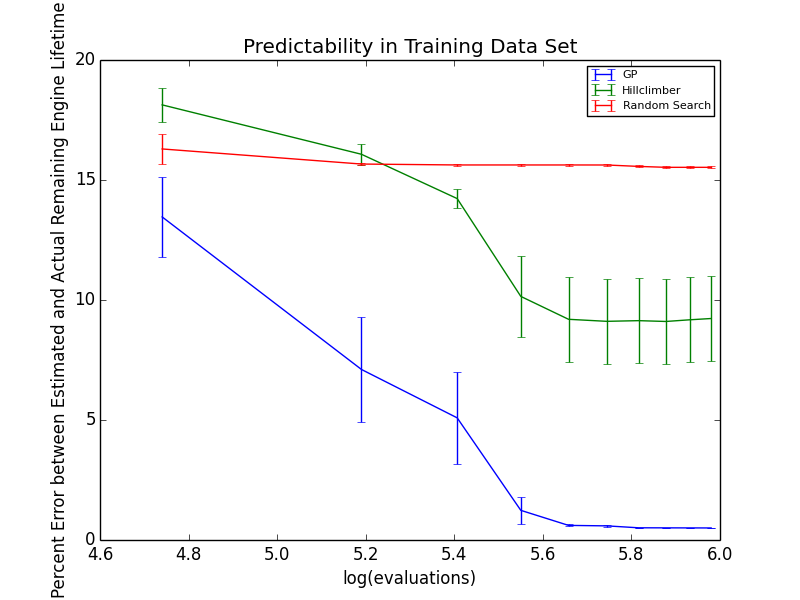
\includegraphics[scale=0.65]{bigplot_one_slice.png}
\caption{{\it{Toy Problem}}: Percent error between estimated and true remaining engine lifetimes in the training data set. Shows GP finding the optimal solution constructed for the toy problem.}
\end{figure*}

\begin{figure*}
\centering
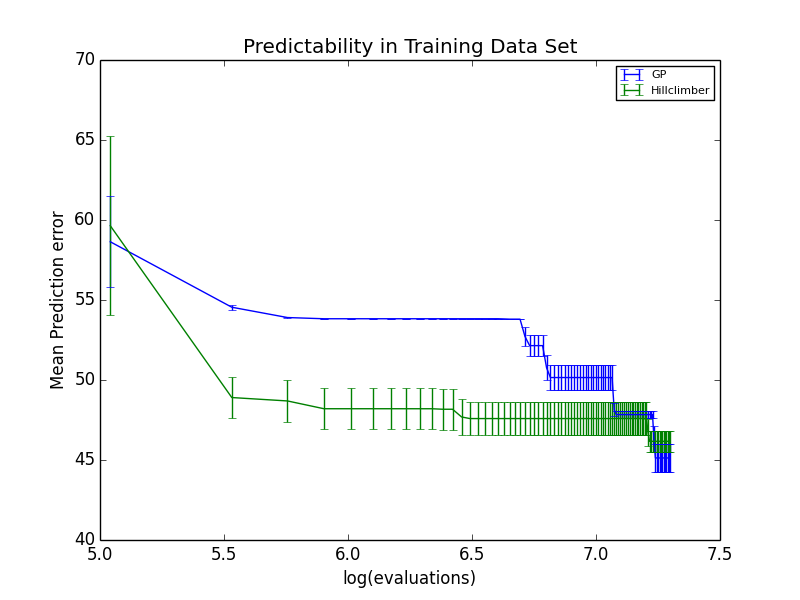
\includegraphics[scale=0.65]{bigplot_2k.png}
\caption{{\it{Real Problem}}: Percent error between estimated and true remaining engine lifetimes in the training data set. GP loses some advantage over hill climber. Y axis is average difference between true and estimated number of remaining engine life cycles.}
\end{figure*}

\begin{figure*}
\centering
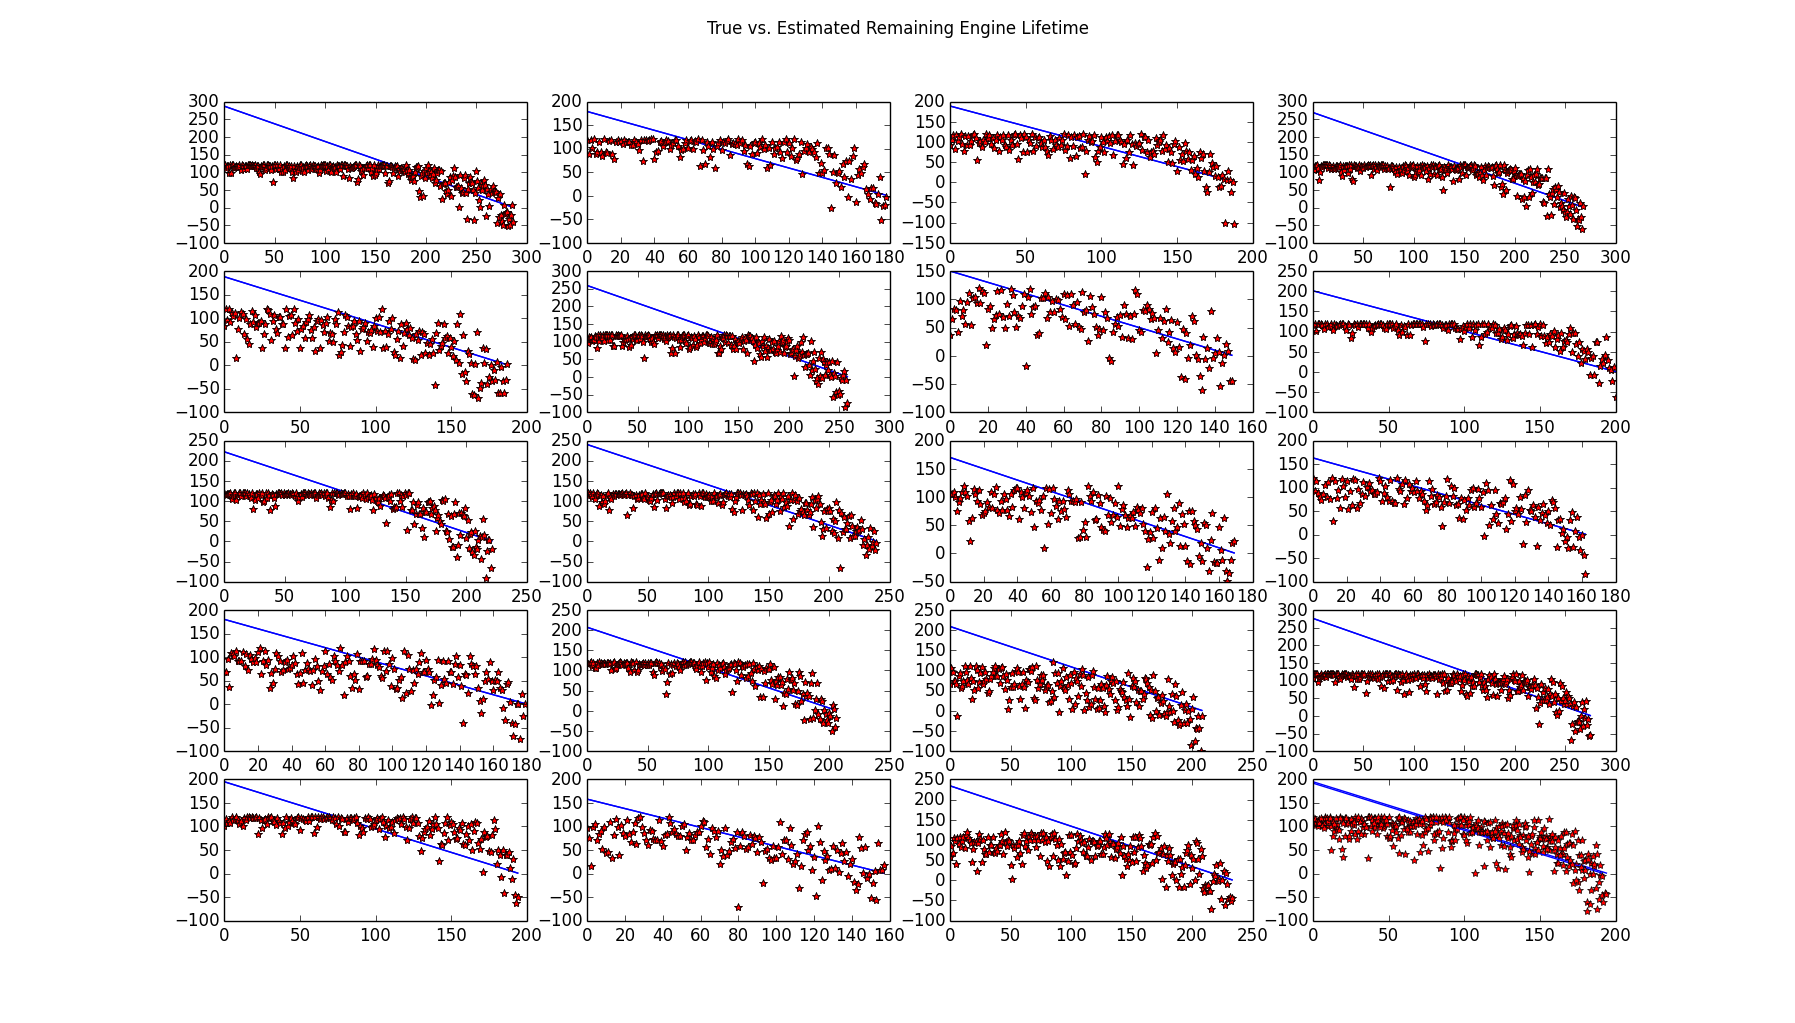
\includegraphics[scale=0.35]{first_20.png}
\caption{{\it{Real Problem}}: Estimated vs. actual remaining engine lifetime. GP has successfully captured the moment of each engine's failure.}
\end{figure*}

\begin{figure*}
\centering
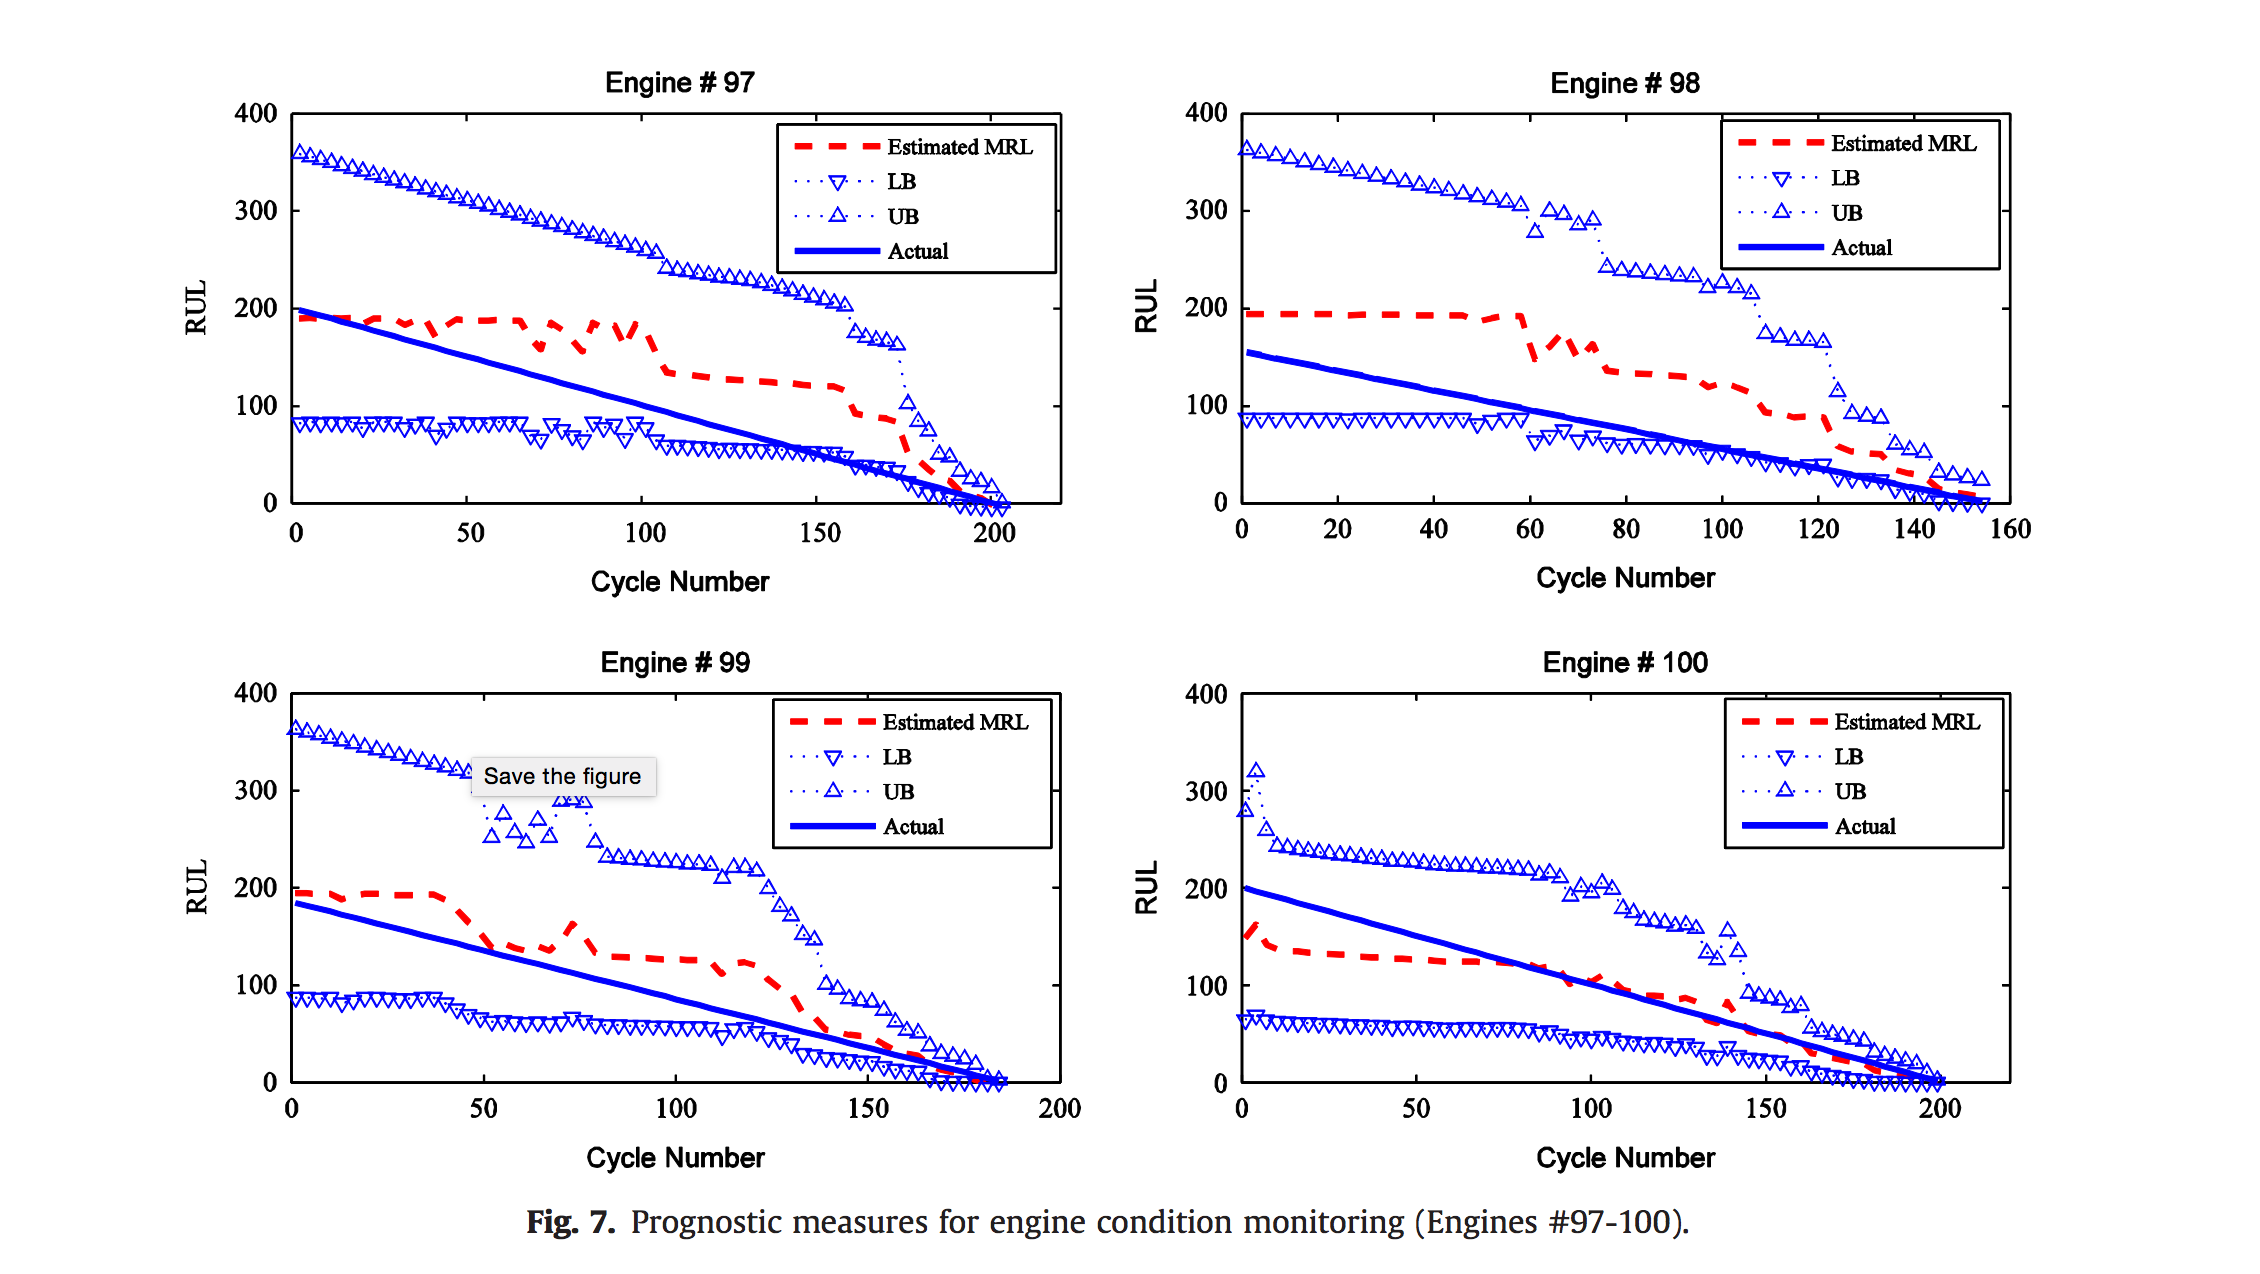
\includegraphics[scale=0.45]{benchmark.png}
\caption{{\it{Real Problem}}: Solutions generated by Moghaddass and Zuo. \cite{Mog}}
\end{figure*}


\subsection{Discussion}
The GP matched Moghaddass and Zuo in prediction accuracy, and it was able to determine the moment of failure for each engine tested. Although the GP's advantage over the hill climber lessened in the real problem (as opposed to the toy problem), the GP did a better job characterizing engine failure in both situations.

The correlation that the GP isolated as being indicative of engine failure is the difference between the outputs of sensors 23 and 6. It was able to use this information to determine when each engine failed, and the remaining lifetime after failure.

\section{Future Work}
There are a couple ways that the performance of the genetic program could likely be improved. 

Currently, fitness for each function in the population is evaluated on every engine in the fleet. By instead representing the fleet of engines as a population, and co-evolving a subset of engines for testing the fitness of each function, the GP would likely converge to a solution with less prediction error more quickly. A fit engine in the engines population would create disagreement among the functions in the solution population.

It is also possible that the GP will do a good job answering a question that is different from the one I asked. Instead of asking for a number corresponding to the remaining engine lifetime, it may be possible to ask for a boolean that answers the question "will this engine fail in the next $x$ cycles?"

\section{Conclusion}
I have demonstrated that symbolic regression is an appropriate technique for data prognostics. The genetic program successfully identified the moment of failure in each engine in the test fleet, and accurately predicted the remaining lifetimes of each of those engines after failure. The method used here matched the non-homogenous continuous-time semi-Markov processing used by Moghaddass and Zuo \cite{Mog}.

Symbolic regression's ability to predict remaining engine lifetime {\it{prior}} to failure is relatively weak, but this is to be expected because no trends would have yet manifested themselves in the data.

%\section{References}
\begin{thebibliography}{99}
%\cite{Clowe:2006eq}
\bibitem{Mog}
Moghaddass, R., & Zuo, M. J. (2014). An integrated framework for online diagnostic and prognostic health monitoring using a multistate deterioration process. Reliability Engineering & System Safety, 124, 92-104.
\bibitem{class}
Lipson, H. (Director) (2014, September 1). Evolutionary Computation. CS 5724. Lecture conducted from Cornell University, Ithaca.
\bibitem{symbolic}
Schmidt, M., & Lipson, H. (2010). Symbolic regression of implicit equations. In Genetic Programming Theory and Practice VII (pp. 73-85). Springer US.
\bibitem{oil}
Byington, C. S., Mackos, N. A., Argenna, G., Palladino, A., Reimann, J., & Schmitigal, J. (2012). Application of symbolic regression to electrochemical impedance spectroscopy data for lubricating oil health evaluation. ARMY TANK AUTOMOTIVE RESEARCH DEVELOPMENT AND ENGINEERING CENTER WARREN MI.
\bibitem{nasa}
Overview. (2008, January 1). Retrieved November 1, 2014, from http://ti.arc.nasa.gov/tech/dash/pcoe/prognostic-data-repository/
\bibitem{nutonian}
Nutonian, Inc. (2011, January 1). Retrieved December 14, 2014, from http://www.nutonian.com/products/eureqa/

\bibitem{pareto}
Deb, K., Agrawal, S., Pratap, A., & Meyarivan, T. (2000). A fast elitist non-dominated sorting genetic algorithm for multi-objective optimization: NSGA-II. Lecture notes in computer science, 1917, 849-858.

\bibitem{horn}
Horn, J., Nafpliotis, N., & Goldberg, D. E. (1994, June). A niched Pareto genetic algorithm for multiobjective optimization. In Evolutionary Computation, 1994. IEEE World Congress on Computational Intelligence., Proceedings of the First IEEE Conference on (pp. 82-87). Ieee.

\section{Acknowledgements}
\begin{itemize}
\item Dr. Hod Lipson and the CS 5724 class, for teaching me all the necessary skills for conducting this research and providing guidance.
\item Andrew Crego of MOOG, for pointing out that deviations in sensor correlation would be a good way of performing data prognostics.
\item Nelson Conover for proof reading my report.
\end{itemize}

\section{Appendix}
A list of filenames included in report, and content:
\begin{itemize}
\item Hunter\_Adams.pdf: Project report
\item treeclass.py: Class and class method definitions
\item finch.py: Initializations, data loading
\item train\_FD001.txt: training data
\item test\_FD001.txt: test data
\item RUL\_FD001.txt: correct answers
\end{itemize}

\balancecolumns
% That's all folks!
\end{document}
